\documentclass[11pt,compress,t,notes=noshow, xcolor=table]{beamer}
\usepackage[]{graphicx}\usepackage[]{color}
% maxwidth is the original width if it is less than linewidth
% otherwise use linewidth (to make sure the graphics do not exceed the margin)
\makeatletter
\def\maxwidth{ %
  \ifdim\Gin@nat@width>\linewidth
    \linewidth
  \else
    \Gin@nat@width
  \fi
}
\makeatother

\newcommand{\citebutton}[2]{%
\beamergotobutton{\href{#2}{#1}}%
}

\newcommand{\blu}[1]{\textcolor{blue}{#1}}
\newcommand{\org}[1]{\textcolor{orange}{#1}}
\newcommand{\ques}{\textbf{\textcolor{red}{Question:  }}}
\newcommand{\questionssofar}{\begin{frame}\frametitle{Any questions?}\end{frame}}

\newcommand\warning{%
 \makebox[1.4em][c]{%
 \makebox[0pt][c]{\raisebox{.1em}{\scriptsize!}}%
 \makebox[0pt][c]{\color{red}\normalsize$\bigtriangleup$}}}%

\definecolor{fgcolor}{rgb}{0.345, 0.345, 0.345}
\newcommand{\hlnum}[1]{\textcolor[rgb]{0.686,0.059,0.569}{#1}}%
\newcommand{\hlstr}[1]{\textcolor[rgb]{0.192,0.494,0.8}{#1}}%
\newcommand{\hlcom}[1]{\textcolor[rgb]{0.678,0.584,0.686}{\textit{#1}}}%
\newcommand{\hlopt}[1]{\textcolor[rgb]{0,0,0}{#1}}%
\newcommand{\hlstd}[1]{\textcolor[rgb]{0.345,0.345,0.345}{#1}}%
\newcommand{\hlkwa}[1]{\textcolor[rgb]{0.161,0.373,0.58}{\textbf{#1}}}%
\newcommand{\hlkwb}[1]{\textcolor[rgb]{0.69,0.353,0.396}{#1}}%
\newcommand{\hlkwc}[1]{\textcolor[rgb]{0.333,0.667,0.333}{#1}}%
\newcommand{\hlkwd}[1]{\textcolor[rgb]{0.737,0.353,0.396}{\textbf{#1}}}%
\let\hlipl\hlkwb

\usepackage{framed}
\makeatletter
\newenvironment{kframe}{%
 \def\at@end@of@kframe{}%
 \ifinner\ifhmode%
  \def\at@end@of@kframe{\end{minipage}}%
  \begin{minipage}{\columnwidth}%
 \fi\fi%
 \def\FrameCommand##1{\hskip\@totalleftmargin \hskip-\fboxsep
 \colorbox{shadecolor}{##1}\hskip-\fboxsep
     % There is no \\@totalrightmargin, so:
     \hskip-\linewidth \hskip-\@totalleftmargin \hskip\columnwidth}%
 \MakeFramed {\advance\hsize-\width
   \@totalleftmargin\z@ \linewidth\hsize
   \@setminipage}}%
 {\par\unskip\endMakeFramed%
 \at@end@of@kframe}
\makeatother

\definecolor{shadecolor}{rgb}{.97, .97, .97}
\definecolor{messagecolor}{rgb}{0, 0, 0}
\definecolor{warningcolor}{rgb}{1, 0, 1}
\definecolor{errorcolor}{rgb}{1, 0, 0}
\newenvironment{knitrout}{}{} % an empty environment to be redefined in TeX

\usepackage{alltt}
\newcommand{\SweaveOpts}[1]{}  % do not interfere with LaTeX
\newcommand{\SweaveInput}[1]{} % because they are not real TeX commands
\newcommand{\Sexpr}[1]{}       % will only be parsed by R
\newcommand{\xmark}{\ding{55}}%


\usepackage[english]{babel}
\usepackage[utf8]{inputenc}

\usepackage{dsfont}
\usepackage{verbatim}
\usepackage{amsmath}
\usepackage{amsfonts}
\usepackage{amssymb}
\usepackage{bm}
\usepackage{csquotes}
\usepackage{multirow}
\usepackage{longtable}
\usepackage{booktabs}
\usepackage{enumerate}
\usepackage[absolute,overlay]{textpos}
\usepackage{psfrag}
\usepackage{algorithm}
\usepackage{algpseudocode}
\usepackage{eqnarray}
\usepackage{arydshln}
\usepackage{tabularx}
\usepackage{placeins}
\usepackage{tikz}
\usepackage{setspace}
\usepackage{colortbl}
\usepackage{mathtools}
\usepackage{wrapfig}
\usepackage{bm}
\usepackage{amsmath}
\usepackage{pifont}

\usetikzlibrary{shapes.multipart,shapes,arrows,automata,positioning,calc,chains,trees, shadows}
\tikzset{
  %Define standard arrow tip
  >=stealth',
  %Define style for boxes
  punkt/.style={
    rectangle,
    rounded corners,
    draw=black, very thick,
    text width=6.5em,
    minimum height=2em,
    text centered},
  % Define arrow style
  pil/.style={
    ->,
    thick,
    shorten <=2pt,
    shorten >=2pt,}
}

\tikzstyle{vec}=[draw, rectangle, fill = white, minimum width=5mm, minimum height=1cm, inner sep = 2pt]

\usepackage{subfig}

% Defines macros and environments
\usepackage{../../style/lmu-lecture}


\let\code=\texttt
\let\proglang=\textsf

\setkeys{Gin}{width=0.9\textwidth}

\setbeamertemplate{frametitle}{\expandafter\uppercase\expandafter\insertframetitle}

\usepackage{bbm}
% basic latex stuff
\newcommand{\pkg}[1]{{\fontseries{b}\selectfont #1}} %fontstyle for R packages
\newcommand{\lz}{\vspace{0.5cm}} %vertical space
\newcommand{\dlz}{\vspace{1cm}} %double vertical space
\newcommand{\oneliner}[1] % Oneliner for important statements
{\begin{block}{}\begin{center}\begin{Large}#1\end{Large}\end{center}\end{block}}


%new environments
\newenvironment{vbframe}  %frame with breaks and verbatim
{
 \begin{frame}[containsverbatim,allowframebreaks]
}
{
\end{frame}
}

\newenvironment{vframe}  %frame with verbatim without breaks (to avoid numbering one slided frames)
{
 \begin{frame}[containsverbatim]
}
{
\end{frame}
}

\newenvironment{blocki}[1]   % itemize block
{
 \begin{block}{#1}\begin{itemize}
}
{
\end{itemize}\end{block}
}

\newenvironment{fragileframe}[2]{  %fragile frame with framebreaks
\begin{frame}[allowframebreaks, fragile, environment = fragileframe]
\frametitle{#1}
#2}
{\end{frame}}


\newcommand{\myframe}[2]{  %short for frame with framebreaks
\begin{frame}[allowframebreaks]
\frametitle{#1}
#2
\end{frame}}

\newcommand{\remark}[1]{
  \textbf{Remark:} #1
}


\newenvironment{deleteframe}
{
\begingroup
\usebackgroundtemplate{
\includegraphics[width=\paperwidth,height=\paperheight]{../style/color/red.png}}
 \begin{frame}
}
{
\end{frame}
\endgroup
}
\newenvironment{simplifyframe}
{
\begingroup
\usebackgroundtemplate{
\includegraphics[width=\paperwidth,height=\paperheight]{../style/color/yellow.png}}
 \begin{frame}
}
{
\end{frame}
\endgroup
}\newenvironment{draftframe}
{
\begingroup
\usebackgroundtemplate{
\includegraphics[width=\paperwidth,height=\paperheight]{../style/color/green.jpg}}
 \begin{frame}
}
{
\end{frame}
\endgroup
}
% https://tex.stackexchange.com/a/261480: textcolor that works in mathmode
\makeatletter
\renewcommand*{\@textcolor}[3]{%
  \protect\leavevmode
  \begingroup
    \color#1{#2}#3%
  \endgroup
}
\makeatother





\input{../../latex-math/basic-math.tex}
\input{../../latex-math/basic-ml.tex}

\newcommand{\learninggoals}{
\item Get to know deterministic decoding strategies
\item Learn how text is generated with greedy search and beam search
\item Understand how beam search tries to fix the drawbacks of greedy search
}
\definecolor{texblue}{rgb}{0, 0, 1}
\def\myblue#1{\textcolor{texblue}{#1}}

\title{Decoding Strategies}
% \author{}
\institute{\href{https://slds-lmu.github.io/lecture_dl4nlp/}{slds-lmu.github.io/lecture\_dl4nlp}}
\date{}

\begin{document}
\lecturechapter{Greedy \& Beam Search}
\lecture{Deep Learning for NLP}

% ------------------------------------------------------------------------------

\begin{vbframe}{Greedy Search (1)}
\href{https://codelabsacademy.com/blog/the-beam-search-algorithm-in-the-context-of-natural-language-processing-and-sequence-generation-tasks}{\beamergotobutton{Codelabs Academy}}
\vfill

\begin{itemize}
    \item \textbf{Core idea}: Greedy search selects the word with the highest probability at each timestep, iteratively building the output sequence
    \item \textbf{Exploration of search space}: It explores a single path through the output space, favoring the most probable word at each step without considering future consequences
    \item \textbf{Candidate Sequence}: Only keeps track of the most likely sequence at each step, discarding other possibilities
    \item \textbf{Decision Making}: It makes local decisions based solely on the highest probability at the current step without considering potential longer-term outcomes
\end{itemize}

\vfill
    
\end{vbframe}

% ------------------------------------------------------------------------------

\begin{vbframe}{Greedy Search (2)}

\vfill

\begin{itemize}
    \item The model accepts an input sequence of tokens $x_1, x_2,...,x_N$, which we also call prompt
    \item The model then generates a token at each timestep $t$ until $T$: $y_1,y_2,...,y_T$
    \item In greedy search we choose the token with the highest conditional probability from the vocabulary V
    \item $y_t = argmax_{y \in V}P(y|y_1,y_2,...,y_{t-1},\mathbf{x})$
    \item With $y_t$ being the chosen token at timestep t and $\mathbf{x} = (x_1, x_2,...,x_N)$ being the initial prompt
\end{itemize}

\vfill

\end{vbframe}

% ------------------------------------------------------------------------------

\begin{vbframe}{Greedy Search: Example}
\href{https://d2l.ai/chapter_recurrent-modern/beam-search.html}{\beamergotobutton{d2l book}}

\begin{itemize}
    \item Suppose our vocabulary only has four tokens: $A$, $B$, $C$ and <eos>
\end{itemize}

\begin{figure}
    \centering
    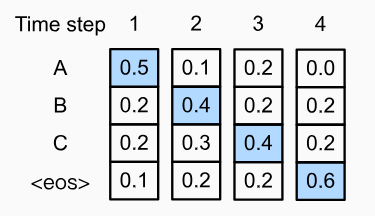
\includegraphics[width=6cm]{chapters/chapter12/figure/greedy.png}
\end{figure}

\begin{itemize}
    \item At each timestep greedy search chooses the token with the highest conditional probability
    \item The model thus predicts $A$, $B$, $C$, <eos>
    \item Its probability is $0.5\cdot 0.4 \cdot 0.4 \cdot 0.6 = 0.048$
\end{itemize}

\end{vbframe}

% ------------------------------------------------------------------------------

\begin{vbframe}{Drawbacks of Greedy Search (1)}

\begin{itemize}
    \item Now we select token $C$ at timestep 2 instead of $B$
\end{itemize}

\begin{figure}
    \centering
    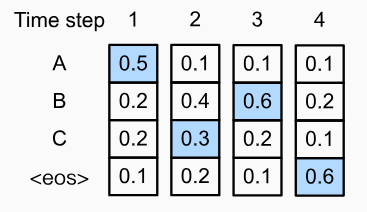
\includegraphics[width=6cm]{chapters/chapter12/figure/greedy2.png}
\end{figure}

\begin{itemize}
    \item At the timesteps 3 and 4 the conditional probabilities change since the context is no longer $A$, $B$ but $A$, $C$
    \item The final token sequence is $A$, $C$, $B$, <eos>
    \item Its probability is $0.5 \cdot 0.3 \cdot 0.6 \cdot 0.6 = 0.054$
    \item Even though $C$ at $t=2$ has a lower probability, the final sequence has a higher probability
\end{itemize}
    
\end{vbframe}

% ------------------------------------------------------------------------------

\begin{vbframe}{Drawbacks of Greedy Search (2)}

\vfill

\begin{itemize}
    \item \textbf{Suboptimal Global Solutions}: It makes decisions based only on the highest probability token at each step, often missing globally optimal solutions
    \item \textbf{Lack of Diversity}: It generates repetitive and predictable text, leading to bland outputs
    \item \textbf{Incoherence in Long Sequences}: It may produce incoherent text over longer sequences due to losing track of the overall context
    \item \textbf{Repetitiveness}: The lack of diversity leads to repetitive phrases, especially in longer texts
    \item \textbf{Overemphasis on Common Phrases}: It favors common words and phrases, resulting in overly generic outputs
\end{itemize}

\vfill

\end{vbframe}

% ------------------------------------------------------------------------------

\begin{vbframe}{Beam Search}
\href{https://codelabsacademy.com/blog/the-beam-search-algorithm-in-the-context-of-natural-language-processing-and-sequence-generation-tasks}{\beamergotobutton{Codelabs Academy}}

\vfill

\begin{itemize}
    \item \textbf{Core idea}: Beam search extends the exploration to multiple possible sequences instead of just the most probable one
    \item \textbf{Exploration of search space}: It explores multiple paths (or "beams") simultaneously, maintaining a set of promising candidate sequences
    \item \textbf{Candidate Sequence}: Keeps a fixed number of most probable sequences (determined by the beam width parameter $k$) at each step
    \item \textbf{Decision Making}: At each step, it considers multiple candidate sequences and selects the most probable ones based on their cumulative probabilities up to that point
\end{itemize}

\vfill

\end{vbframe}

% ------------------------------------------------------------------------------

\begin{vbframe}{Beam Search: Example (1)}
\href{https://d2l.ai/chapter_recurrent-modern/beam-search.html}{\beamergotobutton{d2l book}}

\vfill

\begin{itemize}
    \item Suppose $V = \{A, B, C, D, E\}$ and beam width $k=2$
\end{itemize}

\begin{figure}
    \centering
    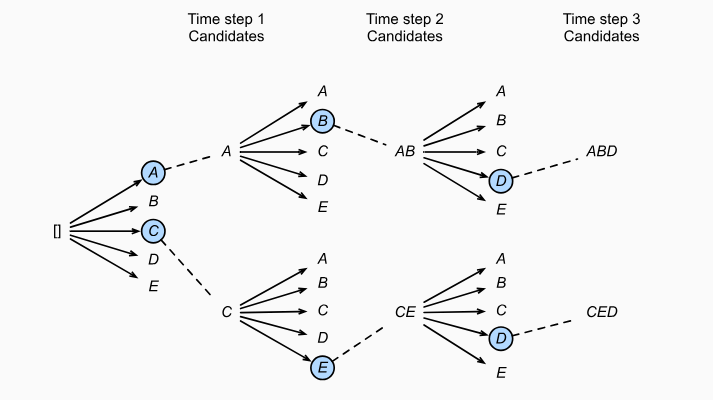
\includegraphics[width=10cm]{figure/beam.png}
\end{figure}

\vfill
    
\end{vbframe}

% ------------------------------------------------------------------------------
\begin{vbframe}{Beam Search: Example (2)}

\vfill

\begin{itemize}
    \item At each timestep beam search chooses the $k$ tokens with the highest joint probability
    \item Suppose at $t=1$ $A$ and $C$ have the highest conditional probabilities $P(y_1|\mathbf{x})$
    \item At $t=2$ for all $y_2\in V$ we compute:
    $$
    \begin{aligned}
    P(A,y_2|\mathbf{x}) &= P(A|\mathbf{x})\cdot P(y_2|A,\mathbf{x}) \\
    P(C,y_2|\mathbf{x}) &= P(C|\mathbf{x})\cdot P(y_2|C,\mathbf{x})
    \end{aligned}
    $$
    \item And we again pick the $k$ sequences with the highest probabilities ($AB$ and $CE$)
    \item At $t=3$ again for all $y_3\in V$ we compute:
    $$
    \begin{aligned}
    P(A,B,y_2|\mathbf{x}) &= P(A,B|\mathbf{x})\cdot P(y_2|A,B,\mathbf{x}) \\
    P(C,E,y_2|\mathbf{x}) &= P(C,E|\mathbf{x})\cdot P(y_2|C,E,\mathbf{x})
    \end{aligned}
    $$
    \item We repeat this process unitl the maximum length is reached or unitl the <EOS> token gets generated
\end{itemize}

\vfill
    
\end{vbframe}

% ------------------------------------------------------------------------------

% \begin{vbframe}{Generate Function \citebutton{G\MakeLowercase{eneration}C\MakeLowercase{onfig}}{https://huggingface.co/docs/transformers/v4.40.0/en/main_classes/text_generation#transformers.GenerationConfig}}

% \vfill

% \begin{itemize}
%     \item The default decoding strategy for \texttt{generate()} is greedy search
%     \item In order to use beam search you have to provide the \texttt{num\_beams} hyperparameter
% \end{itemize}


% \vfill
    
% \end{vbframe}

% ------------------------------------------------------------------------------

\begin{vbframe}{Greedy Search versus Beam Search}

\vspace{2ex}
\textbf{Prompt: "Once upon a time"}
\begin{itemize}
\item Greedy search: \textit{", the United States was the world's leading producer of oil and natural gas. Today, we are the world's leading producer of coal. 
The United States is the world's largest producer of oil and natural gas"}
\item Beam search (beam-width 2): \textit{", I had a friend who was a big fan of the show. He was a huge fan of the show, and I was a huge fan of the show. We would talk about the show all the time"}
\end{itemize}
\vspace{2ex}
The generated stories are repetitive, also referred to as \textit{degenerate}. These decoding strategies don't seem to work well for the task, where more creativity and diversity might be desirable.\\
\vspace{2ex}



\end{vbframe}

% ------------------------------------------------------------------------------

\begin{frame}{Beam Search vs. Human}

\citebutton{Holtzmann et al., 2019}{https://arxiv.org/abs/1904.09751}
\begin{center}
    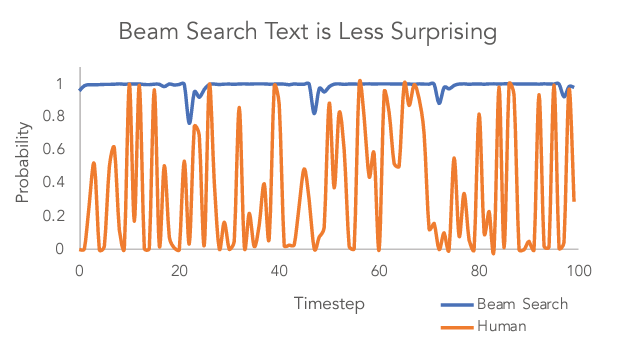
\includegraphics[width=0.7\linewidth]{figure/beam_vs_human.png}
\end{center}

\begin{itemize}
    \item Humans typically use words that have a low probabililty
    \item Beam search though mostly outputs words which have a high probability
\end{itemize}

\vfill

$\Rightarrow$ Incorporate some randomness (next chapter)

\end{frame}


% ------------------------------------------------------------------------------

\endlecture
\end{document}